\documentclass[a4paper]{article}

%% Language and font encodings
\usepackage[T1]{fontenc}
\usepackage[utf8x]{inputenc}
\usepackage[english]{babel}

\usepackage[colorlinks=true, allcolors=blue]{hyperref}

\urlstyle{tt}
\newcommand{\email}[1]{\href{mailto:#1}{\tt{\nolinkurl{#1}}}}
\newcommand{\orcid}[1]{ORCID: \href{https://orcid.org/#1}{\tt{\nolinkurl{#1}}}}

\newcommand{\figleg}[1]{\centering\itshape{#1}\/}
\newcommand{\figref}[1]{(see figure~\ref{#1})}
\newcommand{\secref}[1]{(see~\ref{#1})}

\usepackage[sfdefault,lf]{carlito}

%% The 'lf' option for lining figuressy
%% The 'sfdefault' option to make the base font sans serif
\usepackage[parfill]{parskip}
\renewcommand*\oldstylenums[1]{\carlitoOsF#1}%
\usepackage{fancyhdr}
\usepackage{natbib}
\usepackage{authblk}
\setlength{\headheight}{41pt}

%% Sets page size and margins
\usepackage[a4paper,top=3cm,bottom=2cm,left=3cm,right=3cm,marginparwidth=1.75cm]{geometry}

%% Useful packages
\usepackage{amsmath}
\usepackage{amssymb}
\usepackage{graphicx}
\usepackage{booktabs}
\usepackage{caption}
\usepackage{subcaption}

\usepackage[colorinlistoftodos]{todonotes}

\fancyhead[L]{Posted: \today}
%\fancyhead[R]{
\includegraphics[width=4cm]{img/engrXiv_banner.png}}
\pagestyle{plain}
\title{Causal Comb Filters for Removal of Non-Stationary and Non-Sinusoidal Transcranial Alternating Current Stimulation Artifacts}
\author[1,*]{Robert Guggenberger}
\author[1]{N.N.}
\affil[1]{Department for Translational Neurosurgery, University Hospital Tübingen}

\affil[*]{Corresponding author: \email{robert.guggenberger@posteo.eu}}
\date{\today}

\usepackage{varioref}
\usepackage{hyperref}
\usepackage{cleveref}
\hypersetup{hidelinks = true}
\usepackage{listings}
\usepackage{Matlab-prettifier}
\usepackage[nonumberlist,acronym]{glossaries}
% abbreviations:
\newacronym{eeg}{EEG}{electroencephalogram}
\newacronym{ecg}{ECG}{electrocardiogram}
\newacronym{tacs}{tACS}{transcranial alternating current stimulation}
\newacronym{tms}{TMS}{transcranial magnetic stimulation}
\newacronym{tpca}{tPCA}{temporal principal component analysis}
\newacronym{ppca}{pPCA}{periodic principal component analysis}
\newacronym{sma}{SMA}{superposition of moving averages}
\newacronym{erp}{ERP}{event-related potential}
\makeglossaries{}

% --------------------------------------------------------------------------
\begin{document}
\maketitle
\thispagestyle{fancy}

\begin{abstract}
We present motivation and justification for weighted causal comb filters with the goal to remove non-stationary and non-sinusoidal artifacts of transcranial alternating current stimulation from electrophysiological recordings.
We evaluate predefined (uniform, linear, exponential, gaussian) or empirical (periodic autocorrelation) weighting functions, and contrast them with symmetric uniform comb filters, discrete Fourier filters and periodic principal component removal.
Evaluation is performed using simulated data and electrophysiological recordings certain to show no physiological modulation by the stimulation, i.e. R-peaks recorded from the upper left arm.
We found that all approaches were similarily able to recover the signal. Noteworthy for real-time environments with limited computational power is that the causal uniform filter is comparable to computationally more complex approaches.
Yet, note the issue of echos, which can only partially be countered by~\emph{convex} weights and limit the applicablity of comb filters to physiological signals with a duration less than one period of the artifact.
Finally, note that comb filters are purely periodic with no assumptions about the shape of the artifact. Comb filters might therefore be useful for filtering of deliberately non-sinusoidal transcranial current stimulation.
The filters were implemented as module for Matlab 2016b. The code can be accessed online at \url{https://github.com/agricolab/ARtACS} under a X11-license.

\end{abstract}

\section{Introduction}

The combination of \gls{tacs} and \gls{eeg} has been explored in several recent studies. While the analysis of \gls{eeg} before or after stimulation posits limited technical challenges, the \gls{eeg} recording during stimulation is heavily affected by the stimulation artifact. This has been linked to the spatial distribution, the non-stationary amplitude and the distorted sinusoidality of the artifact.

\subsection{Spatial Covariance}

It has been argued that unregularized spatial filters might be able to remove the stimulation artifact~\citep{Neuling_2017}. But if only few channels are recorded, the estimation of the spatial covariance can be insufficient. In the single-channel-case, spatial filters are impossible.
Additionally, it has been reported that the spatial covariance is itself not stationary and that the artifact encompasses a large spatial subspace~\citep{Noury_2016}.

\subsection{Non-Stationary Amplitude Modulation}

Consider the assumption that the artifact is stationary and superpositioned on the physiological signal.
Then, modulations in the amplitude of the recorded~\gls{eeg}-signal must be caused by changes in the underlying physiology.
This would be the case, even if frequency and phase are matched to the stimulation signal. Approaches assuming such stationarity of the stimulation artifact have been used e.g.\ by~\cite{Pogosyan_2009}.

Yet, practical experience suggests that the stimulation artifact is actually not stationary~\figref{fig:nonstationary}.
As a recording can exhibit an amplitude modulation of the stimulation artifact when the clocks of stimulation and recording device are not synchronized, this has been suggested as a cause for amplitude modulations.
It has also been suggested that the closed-loop current control process within the stimulator might be a further source of amplitude modulation~\citep{Neuling_2017}.
Additionally, the amplitude has been reported to by modulated by heart-beat and respiration~\citep{Noury_2016}. Event-related modulation of skin impedance can also affect the scalp conductance at stimulation electrodes.

\subsection{Artifact Distortion}

Ideally, the stimulation artifict of~\gls{tacs} resembles a sinusoid. But practical experience suggests that the signal is often distorted to various degrees.
Figure~\ref{fig:nonsinus} shows examples of distortion and saturation in two recordings of \gls{tacs}. The gray traces indicate nine invididual artifact periods, while the red trace indicates their average. In figure~\ref{fig:distortion}, note the periodic, yet non-sinusoidal waveform. In figure~\ref{fig:saturation}, note the saturation.

The temporally and spatially uneven impedance distribution has been suggested as cause of distortion.
Additionally, non-linearites in the amplifier slew rate can distort the shape when the signal is close to the saturation threshold.
But a major source of possible distortion can be  amplifier saturation, i.e.\ the stimulation artifact exhibiting an amplitude to large for the dynamic range of the amplifier, causing the signal to be cut off. As information is lost, it is impossible to recover signals during periods of saturation.

\begin{figure}[hbtp]
    \begin{subfigure}{1\textwidth}
    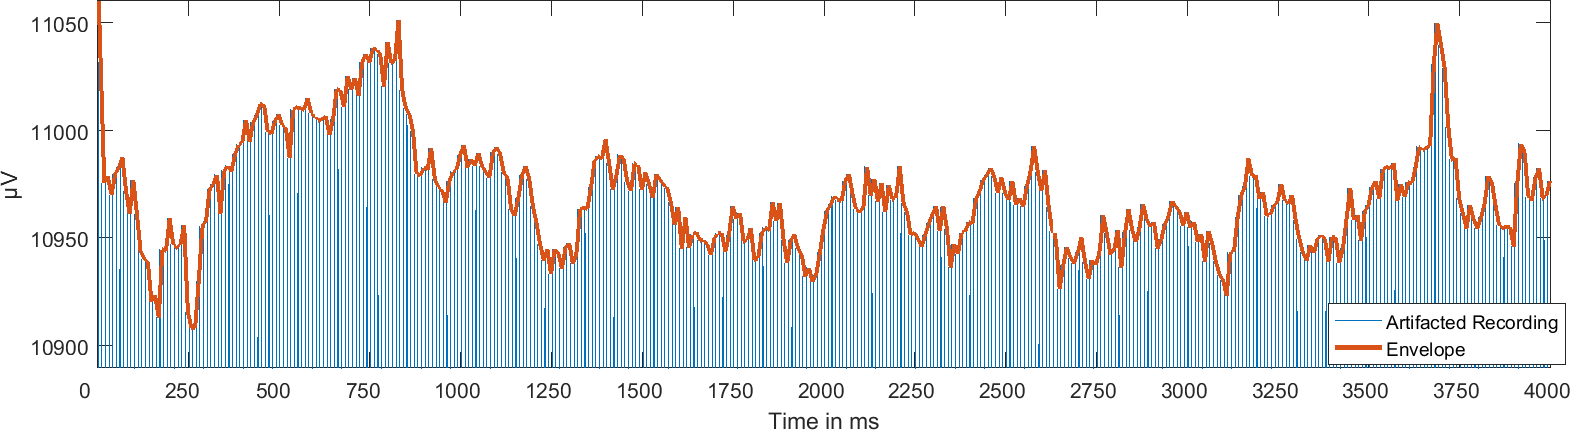
\includegraphics[width=\textwidth]{./img/intro/nonstationarity.png}
    \caption{Non-Stationary Amplitude Modulation}\label{fig:nonstationary}
    \end{subfigure}

    \begin{subfigure}{.5\textwidth}
    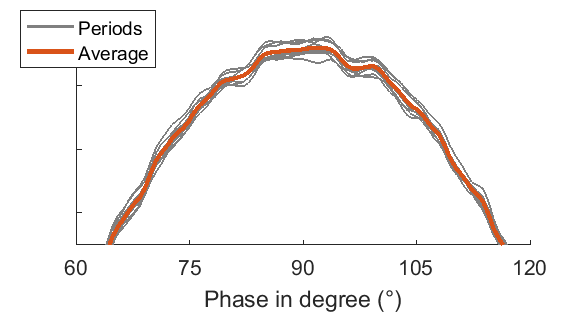
\includegraphics[width=\textwidth]{./img/intro/distortion.png}
    \caption{Distortion}\label{fig:distortion}
    \end{subfigure}
    \begin{subfigure}{.5\textwidth}
    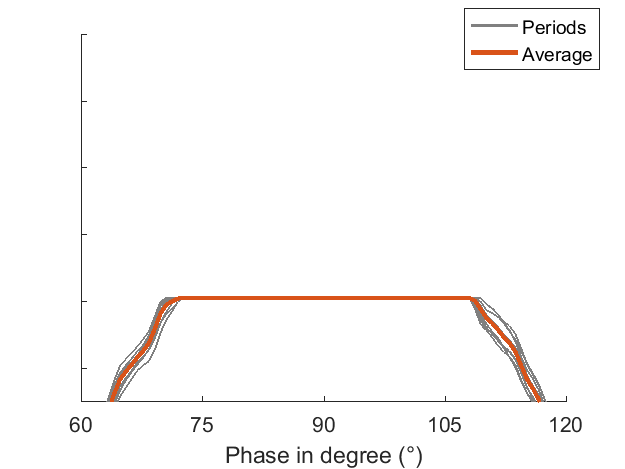
\includegraphics[width=\textwidth]{./img/intro/saturation.png}
    \caption{Saturation}\label{fig:saturation}
    \end{subfigure}

    \caption{Exemplary Recordings highlight Distortion and Non-Stationarity}\label{fig:nonsinus}
\end{figure}

\subsection{Computational Demands}

Methods based on adaptive template construction and \gls{tpca}~\citep{Niazy_2005} have been explored for removal of  non-stationary and misshaped \gls{tacs} artifacts~\citep{Helfrich_2014}.
Consider that the process of template construction, the estimation of accurate weights for removal by template subtraction and the suqsequent removal of residual artifacts using \gls{tpca} is computationally cumbersome. Additionally, it often requires off-line analysis supported by visual inspection.
Such a multi-staged template-approach is therefore of limited utility for on-line artifact removal, especially in a single-channel case.

\subsection{Motivation}

In conclusion, recovering the true signal from an artifacted recording is technically challenging because the artifact is non-stationary, non-sinusoidal and might exhibit a complex topography. We were interested in development of a computationally fast approach, feasible for online artifact removal in a single channel, and usable in embedded systems with limited computational power.
Nonetheless, the implementation was desired to be feasible for offline-analysis. First, to be usable for already recorded datasets and second, to allow reproducible evaluation and comparison with other techniques.

\section{Approach}

The main idea is that at any given time point $t$, the recorded signal $r(t)$ is a linear super\-position of a neurophysiological signal $n(t)$, the stimulation artifact $a(t)$ and a white noise term $e(t)$. The task is to recover $n(t)$ by estimating $\hat{a}(t)$ and $e(t)$ and subtracting from $r(t)$.

\begin{eqnarray}
    r(t) = n(t) + a(t) + \epsilon(t)\\
    n(t) = r(t) - \hat{a} - \epsilon(t)
\end{eqnarray}

\subsection{Periodic Estimation}
Assume that the~\gls{tacs} artifact were \emph{non-sinusoidal}, but \emph{stationary and periodic}. At the same time, assume that neurophysiological signals $n$ and noise $\epsilon$ were absent.
Then, we could estimate the amplitude of $a$ at any time-point $t$ by using the signal $r$ recorded from any time-point, as long as this time-point is an integer multiple of the artifacts period length $p$ earlier~\eqref{eq:Comb}.
Subtraction of a delayed version of the signal is also known as comb filter. Please note that for discretely sampled signals, this approach natively supports only frequencies which are integer divisibles of the sampling frequency. If this is not the case, upsampling the recorded signals to an appropriate sampling rate, comb filtering, and downfiltering is a viable approach.

\begin{eqnarray}
    \hat{a}(t) = r(t-np)\label{eq:Comb}\\
    n \in \mathbb{Z}
\end{eqnarray}

\subsubsection{Uniform Comb Filter}

Consider that the noise term $\epsilon$ is still superpositioned on $r$. If the noise term were white, and because the expectation of white noise $\langle\epsilon\rangle$ converges asymptotically to zero with increased sample size, an approach to estimate a bias-free  artifact amplitude would be to average across as many earlier periods as possible~\eqref{eq:Uniform}.
Subsequently, this estimate can be used to  remove the artifact from $r$.
In real applications, stimulation duration is limited and computational constraints exist. This is reflected by the fact that we have to use a finite number for $N$.

\begin{equation}
    \hat{a}(t) = \sum_{n=1}^{N} \frac{r(t - np)}{N}\label{eq:Uniform}
\end{equation}

\subsubsection{Superposition of Moving Averages}\label{sec:sma}

Please note that averaging across neighbouring periods $M$~\eqref{eq:SMA} has been suggested before and termed~\gls{sma} by~\cite{Kohli_2015}.

\begin{equation}
    \hat{a}(t) = \sum_{n-M/2}^{n+M/2} \frac{r(t - np)}{M+1}\label{eq:SMA}
\end{equation}

Consider that the approach using only past values~\eqref{eq:Uniform} returns a causal filter. Applied online, a causal filter would be able to remove the artifact without the delay of $(Mp)/2$ necessary for~\gls{sma}. Furthermore,~\gls{sma} is well-defined only for even $M$. This motivates the exploration of causal filters for artifact removal.

\subsection{Temporal Weighting}

Consider that the amplitude of the  artifact has been described to be non-stationary and dynamically modulated~\citep{Noury_2016,Neuling_2017}.
Although it has been suggested that there are event-dependent components of the amplitude modulation (e.g.\ by heartbeat or respiration~\cite{Noury_2016} or stimulator impedance check~\cite{Neuling_2017}), the parameters of the dynamical system governing event-independent amplitude modulation are usually not known a priori. This can render online artifact removal problematic.

One approach to tackle this problem is to use instead of a constant weight $1/N$~\eqref{eq:Uniform}, a lag-dependent weighting function $w_n$~\eqref{eq:Weighted}.
\begin{equation}
    \hat{a}(t) = \sum_{n=1}^{N} w_n r(t - np)\label{eq:Weighted}
\end{equation}

By controlling the parameters of the weight functions, can we attempt to match the process governing the amplitude modulation
This might allow us to achieve a better artifact estimation and subsequent removal. Please note that if the reliability of past periods can be estimated, we might select weights empirically~\secref{sec:adaptivePCA}.
Yet, these approaches require extended calculation periods and/or offline analysis. In the following sections, we will discuss and justify three predeterminable weighting functions feasible for fast online-filtering.

\subsubsection{Justification by Sampling}
Consider for example the simple one-step comb filter, where we remove the artifact by subtracting a value sampled from any earlier period.
Assume now that this value were not drawn from the last period, but instead drawn at random from the last $N$ periods with uniform distribution.
If the system governing amplitude modulation were fully stationary for the last $N$ periods, performance would in law be virtually identical to the comb filter based on averaging~\eqref{eq:Uniform}.
If it were instead non-stationary, we would expect that the accuracy of the estimate degrades with longer delay while the precision improves by increasing the number of periods on which we base our estimate.
For example, in the case of the uniform filter, we have a shape parameter $N$, defining how far back we trust a measurement to have the same accuracy as earlier samples.
This rationale justifies non-uniform weights, and to use weights that are designed to increase precision and accuracy of the estimate.

\subsubsection{Justification by AR~(1) process}

Consider that the system governing the amplitude of the stimulation artifact could be decomposed into the constant amplitude $c$ controlled by the stimulator and a dynamical, \emph{event-unrelated} process governing the amplitude modulation. If we model this process as an AR~(1) process, this would return for $N$ approaching infinity:

\begin{align}
    X_{t} = c + \sum_{n=0}^{\infty} \phi_n \epsilon_{t-k}\label{eq:AR1process}
\end{align}

If the kernel $\Phi$  behind the modulation of the artifacts amplitude were known, or could be estimated sufficiently, we could construct an optimal weighting function as a deconvolution filter.
This line of reasoning is based on the similarity between the generic weighted comb filter~\eqref{eq:Weighted} and the generic discrete-time AR~(1) process~\eqref{eq:AR1process}.
Note that, for practical applications, we would need finite $N$. This would limit the application to kernels decaying sufficiently fast.

\subsection{Temporal Weighting Examples}

\subsubsection{Linear Weighting}

One straight-forward approach is using a linear decreasing weighting function. The assumption of local linearity is widely used in the analyis of non-linear dynamical systems, which could render the kernel sufficiently flexible.
Additionally, the function is simple and the necessary normalization can easily be calculated by using the triangular number for a given $N$ as normalizing constant $k$~\eqref{eq:NormLinear}.
Hence, equation~\eqref{eq:Linear} returns weights for earlier periods based on a linear temporal weight decay.

\begin{equation}
    w_n = \frac{N-n+1}{k}\label{eq:Linear}
\end{equation}
with the following normalization
\begin{equation}
    k  = \sum_{n=1}^{n} n = \frac{N(N+1)}{2}\label{eq:NormLinear}
\end{equation}

\subsubsection{Exponential Weighting}

Motivated by the fact that the autocorrelation function of an AR~(1) process can be expressed as a decaying exponential, an alternative approach would be an exponential weighting function.
The time constant $\tau$ of an exponential controls its temporal decay. To maintain the shape across different $N$, we consider it reasonable to normalize $n$ by $N$. Hence, equation~\eqref{eq:Exp} returns weights for earlier periods based on their exponential temporal weight decay.

\begin{equation}
    w_n = \frac{1}{k} e^{\tau-\tau{(n/N)}}\label{eq:Exp}
\end{equation}
with the following normalization
\begin{equation}
    k  = \sum_{n=1}^{N} e^{\tau-\tau{(n/N)}}\label{eq:NormExp}
\end{equation}

\subsubsection{Gaussian Weighting}

Consider that the amplitude modulation might be governed by more than one AR~(1) process, or the process might be non-stationary itself.
Motivated by the fact that such sums  often converge to a normal distribution, an alternative approach would be a Gaussian weighting function.
Using a suitable parameterization, and centering on zero, the inverse of the standard deviation $1/\sigma^2$ defines the time constant $\tau$ of a Gaussian distribution, which controls its temporal decay.
To maintain the shape across different $N$, we consider it again reasonable to normalize $n$ by $N$. Hence, equation~\eqref{eq:Gauss} returns weights for earlier periods based on their Gaussian temporal weight decay.

\begin{equation}
    w_n = \frac{1}{k} f(n/N)\label{eq:Gauss}
\end{equation}
with the following generating function and normalization
\begin{align}
    f(x)  & = \sqrt{\frac{\tau}{2\pi}} e^{-(\tau x^2)/2}  \\
    k  & = \sum_{n=1}^{N} f(n/N)\label{eq:NormGauss}
\end{align}

\subsection{Alternative Filter Approaches}

Besides the discussed real-valued causal comb filters, several other approaches for filtering the~\gls{tacs}-artifact are possible. For example, one could derive the weight at each period from the autocorrelation across periods~\secref{sec:automaticKernel}, or remove periodic principial components until the artifacts power is sufficiently suppressed~\secref{sec:adaptivePCA}, or use complex-valued kernels which would natively support non-integer frequencies~\secref{sec:causalDFT}.

\subsubsection{Automatic Weight Estimation}\label{sec:automaticKernel}

As mentioned, weighted comb filters can be justfied by using  weights to maximize accuracy and precision of the artifact estimate based on sampling from earlier periods.
This process can be put on an empirical foundation, e.g.\ by calculating the autocorrelation of the recording, which is dominated by the artifact. Weights are then based on the autocorrelation coefficients at periodic lags.

\subsubsection{Causal Discrete Fourier Transformation}\label{sec:causalDFT}

We might also tackle the non-stationarity of the artifact by  estimating the artifacts power in a specific frequency for each time-point, using a window of $N$ periods based on the frequency of~\gls{tacs}. This approach can be implemented as convolution of the recording with a complex kernel at the artifacts frequency, followed by subtraction.
While it has the advantage that it supports natively frequencies which are not integer divisibles of the sampling frequency, we need to assume sinusoidality of the artifact. Additionally, to remove the artifact at harmonic frequencies, the computation has to be performed several times for each harmonic frequency.
Whether this approach is sufficient, will therefore depend on whether the artifact can be sufficiently catched by these few frequencies.

\subsubsection{Adaptive Removal of Periodic Principal Components}\label{sec:adaptivePCA}

Instead of understanding the artifacts in sinusoidal terms, we can also focus on its periodicity and estimate the modulation of the artifacts periodic components across time.
This can be implemented by cutting a recording into epochs with period length, followed by prinical component analysis.\footnote{Please note that we found that the naive approach of simply cutting the recording into epochs of period length returned boundary artifacts at the start and end of each epoch. Running the algorithm at a set of random initial lags, and subsequently averaging their results was sufficient to remove such boundary artifacts.}
If the trial duration is significantly larger than the duration of the physiological signal, and as the artifacts amplitude is much larger than the physiological signal, we are justified to assume that the physiological signal will only span a subspace with small eigenvalues.
The major components will catch the shape components of the artifact, their amplitude modulation over time, and if present, any phase-lag induced by clock asynchrony between stimulator and recording devices. Removing the largest principal components will therefore be more likely to reduce the power of the artifact, and not of the signal.
Removal of the largest component derived using main~\gls{ppca} can be performed iteratively until a specific condition is achieved. We implemented such an iterative approach by removing components until the power in the artifacts main frequency was reduced below the level of nearby, non-artifacted frequencies.

\section{Evaluation}
We implemented all of the discussed approaches for kernel creation and artifact removal in Matlab 2016b. The code can be accessed online~\footnote{\url{https://github.com/agricolab/ARtACS}},free and open source, and has been licensed under a X11-license.

We selected several kernel approaches and evaluated their frequency response characteristics~(see~\ref{sec:EvaluationFreq}). Additonally,we evaluated their performance in comparison also to alternative approaches on simulated~(see~\ref{sec:EvaluationSimulated}) and real data~(see~\ref{sec:EvaluationData}).

\subsection{Evaluation of Frequency Response}\label{sec:EvaluationFreq}

Examine the following exemplary kernels constructed for a sampling rate of 1KHz, a stimulation frequency of 10 Hz and a memory of 10 periods~\figref{fig:ExemplaryCausalKernels}.

\begin{figure}[hbtp]
    \begin{subfigure}{.16\textwidth}
        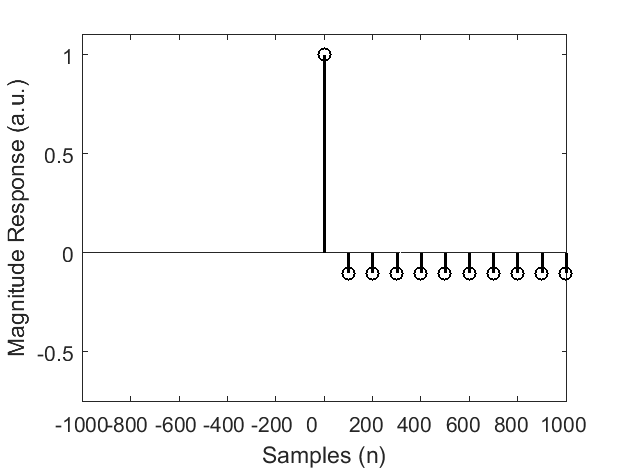
\includegraphics[width=\textwidth]{img/causal/kernel_ave.png}\\
        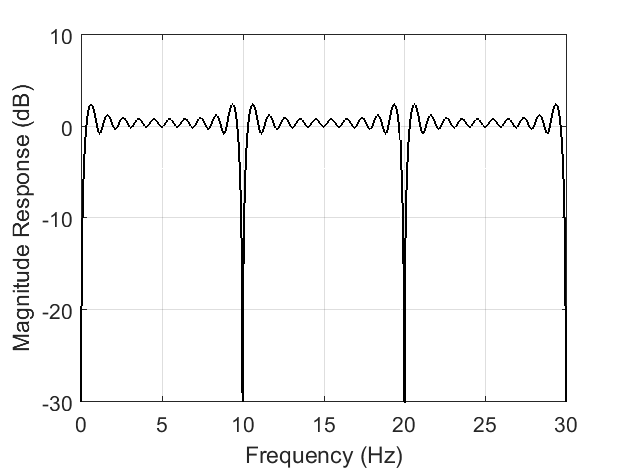
\includegraphics[width=\textwidth]{img/causal/mag_ave.png}
        \caption{\scriptsize{Uniform}}\label{fig:UniformKernel}
    \end{subfigure}
    \begin{subfigure}{.16\textwidth}
        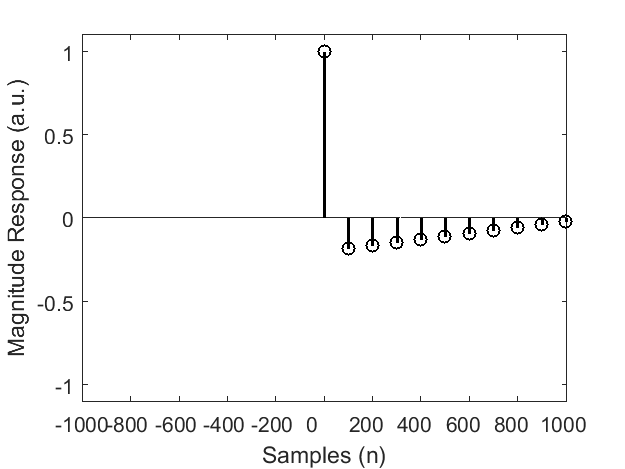
\includegraphics[width=\textwidth]{img/causal/kernel_linear.png}\\
        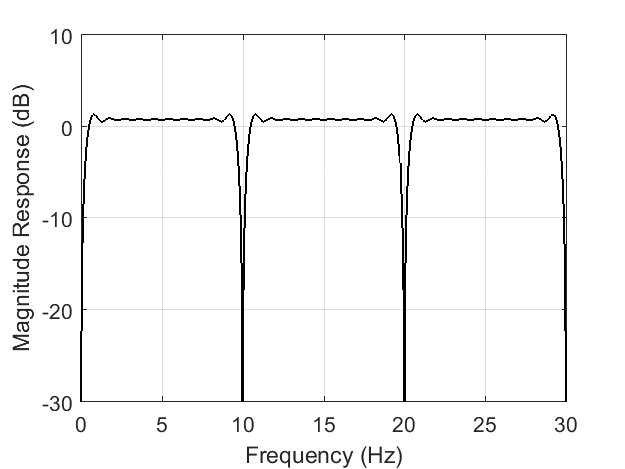
\includegraphics[width=\textwidth]{img/causal/mag_linear.png}
        \caption{\scriptsize{Linear}}\label{fig:LinearKernel}
    \end{subfigure}
    \begin{subfigure}{.16\textwidth}
        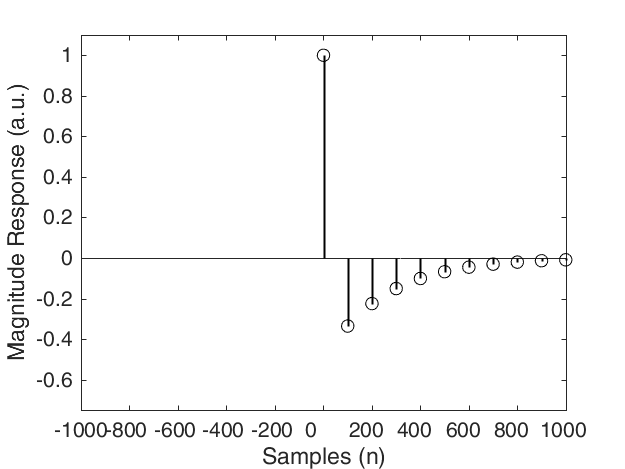
\includegraphics[width=\textwidth]{img/causal/kernel_exp.png}\\
        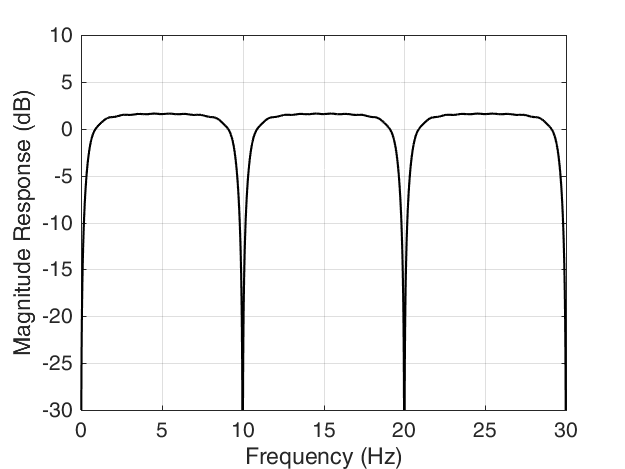
\includegraphics[width=\textwidth]{img/causal/mag_exp.png}
        \caption{\scriptsize{Exponential~$\tau=4$}}\label{fig:ExponentialKernel}
    \end{subfigure}
    \begin{subfigure}{.16\textwidth}
        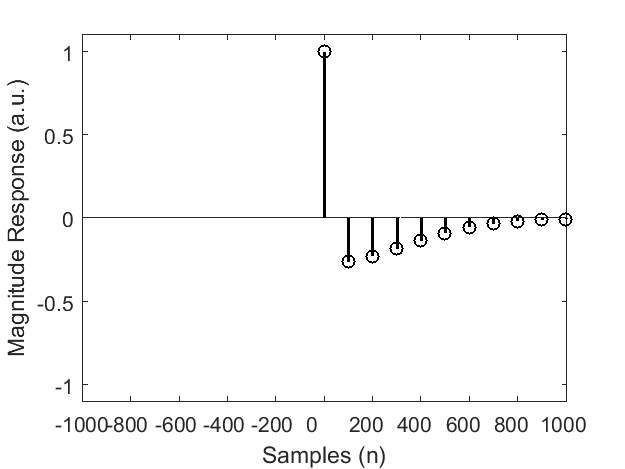
\includegraphics[width=\textwidth]{img/causal/kernel_gauss.png}\\
        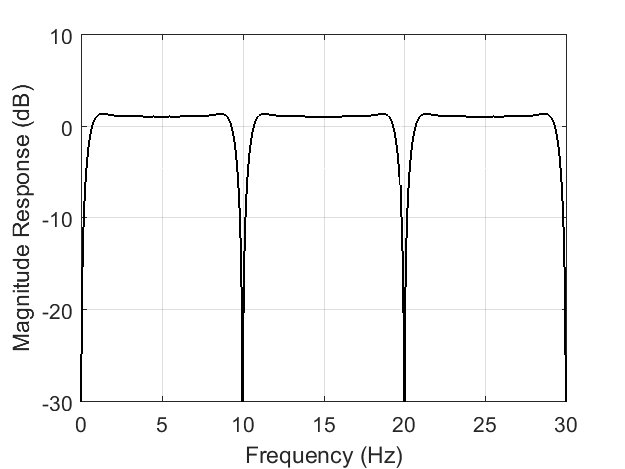
\includegraphics[width=\textwidth]{img/causal/mag_gauss.png}
        \caption{\scriptsize{Gaussian~$\tau=3$}}\label{fig:GaussKernel}
    \end{subfigure}
    \begin{subfigure}{.16\textwidth}
        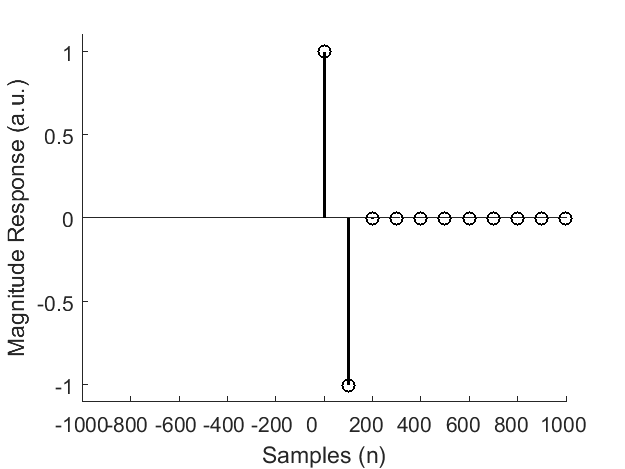
\includegraphics[width=\textwidth]{img/tau/kernel_exp_100.png}\\
        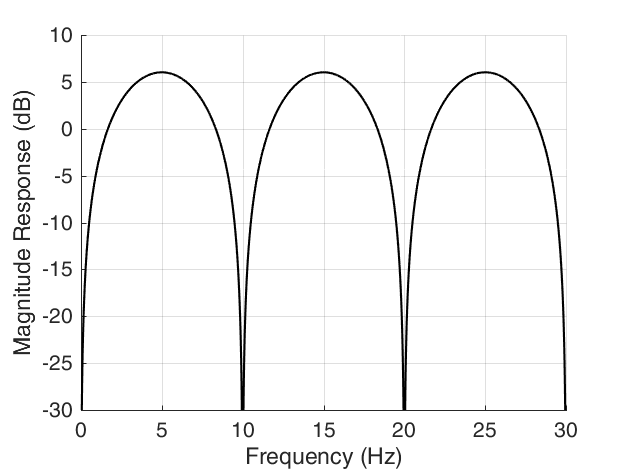
\includegraphics[width=\textwidth]{img/tau/mag_exp_100.png}
        \caption{\scriptsize{Exp~$\tau=100$}}\label{fig:ExpTau100}
    \end{subfigure}
    \begin{subfigure}{.16\textwidth}
        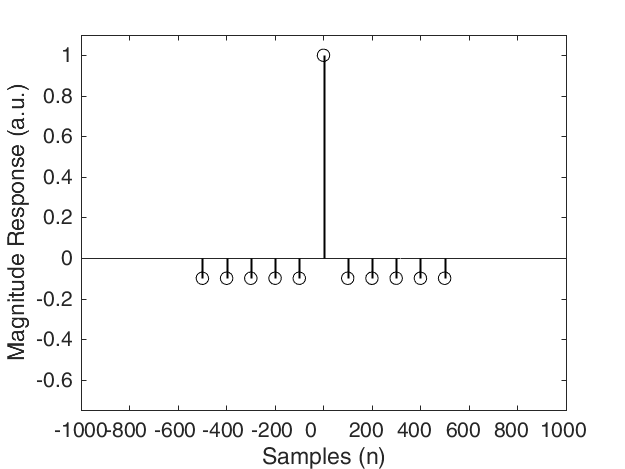
\includegraphics[width=\textwidth]{img/sym/kernel_ave.png}\\
        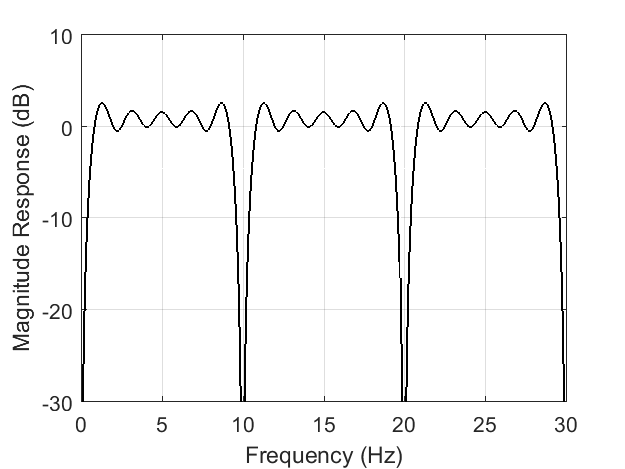
\includegraphics[width=\textwidth]{img/sym/mag_ave.png}
        \caption{\scriptsize{Symmetric Uniform}}\label{fig:SymmetricUniform}
    \end{subfigure}
    \caption{Exemplary Kernels highlight Differences especially in the Pass-band}\label{fig:ExemplaryCausalKernels}
\end{figure}

As you can see from figure~\ref{fig:ExemplaryCausalKernels}, the magnitude responses of the comb filteres approaches are similar in their key characteristic. All exhibit a strong supression of the recordings DC component, the target frequency, and its harmonics.
Yet, note that the filters exhibit strong difference in passband behavior. We find strong ringing in the passband for the uniform~(\ref{fig:UniformKernel}) and linear kernel~(\ref{fig:LinearKernel}), especially compared to the smooth transitions of the exponential~(\ref{fig:ExponentialKernel}) or Gaussian kernel~(\ref{fig:GaussKernel}).
Passband ringing is also present for the~\gls{sma} or symmetric uniform kernel~(\ref{fig:SymmetricUniform}).

We also constructed a set of exponential kernels constructed with different $\tau$ to explore their behavior.
We find it of note that that in the limiting case of $\tau = 0$, the exponential kernel virtually converges with the uniform kernel~\figref{fig:UniformKernel}. Using a $\tau$ equal to the artifacts period length, the exponential kernel almost fully converges with a simple one-step comb filter~\figref{fig:ExpTau100}.
Note also that for all decreasing weight functions, very high $\tau$ would return an impulse response, and therefore just pass all signals.

\subsection{Evaluation on Simulated Signals}\label{sec:EvaluationSimulated}

To evaluate the filters, we tested them on simulated signals. The simulated signal was created as superposition of a 10 Hz \gls{tacs}-artifact, and an \gls{erp}.
The \gls{erp} was simulated as the gradient of a flat top window. The amplitude of the artifact was simulated as a distorted, non-stationary sinusoidal.
The initial stimulation signal was modelled as sinusoidal signal. We distorted it by adding periodic white noise. Additionally, the stimulation amplitude was driven by an Ornstein–Uhlenbeck process with a stiffness 0.5, and a Hanning window time-locked to the event-related potential.
In that way, we were able to simulate event-independent modulations of the artifacts amplitude, and modulations locked to an event.~\footnote{Code for signal generation is included in the toolbox at \url{https://github.com/agricolab/ARtACS}}
Such effects were described by \citep{Noury_2016}, as having a strong potential to mask the true event-related neurophysiological activity.

\begin{figure}[hbtp]
    \begin{subfigure}{0.245\textwidth}
        
\includegraphics[width=\textwidth]{./img/div/desktop_computer.png}
        \caption{Experimental Setup}
    \end{subfigure}
    \begin{subfigure}{0.75\textwidth}
        \begin{subfigure}{.45\textwidth}
            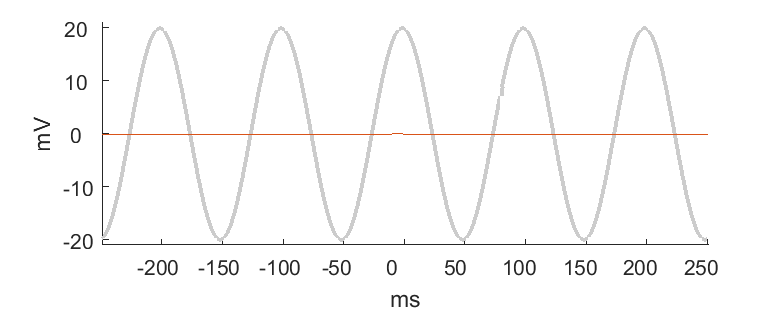
\includegraphics[width=\textwidth]{./img/eva/sim_raw_1.png}
        \end{subfigure}
        \begin{subfigure}{.45\textwidth}
            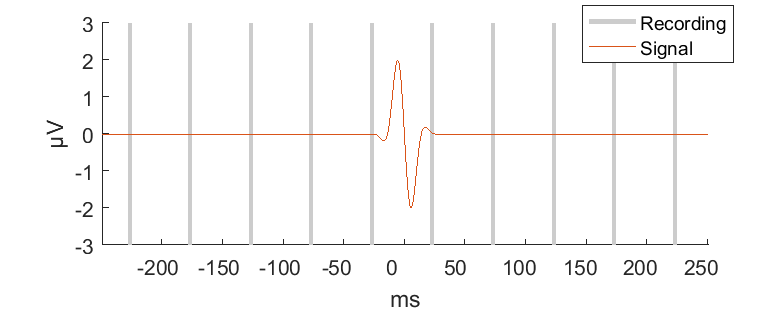
\includegraphics[width=\textwidth]{./img/eva/sim_raw_2.png}
        \end{subfigure}
    \caption{Signal Comparison}\label{fig:simRaw}
    \end{subfigure}
    \begin{subfigure}{1.0\textwidth}
        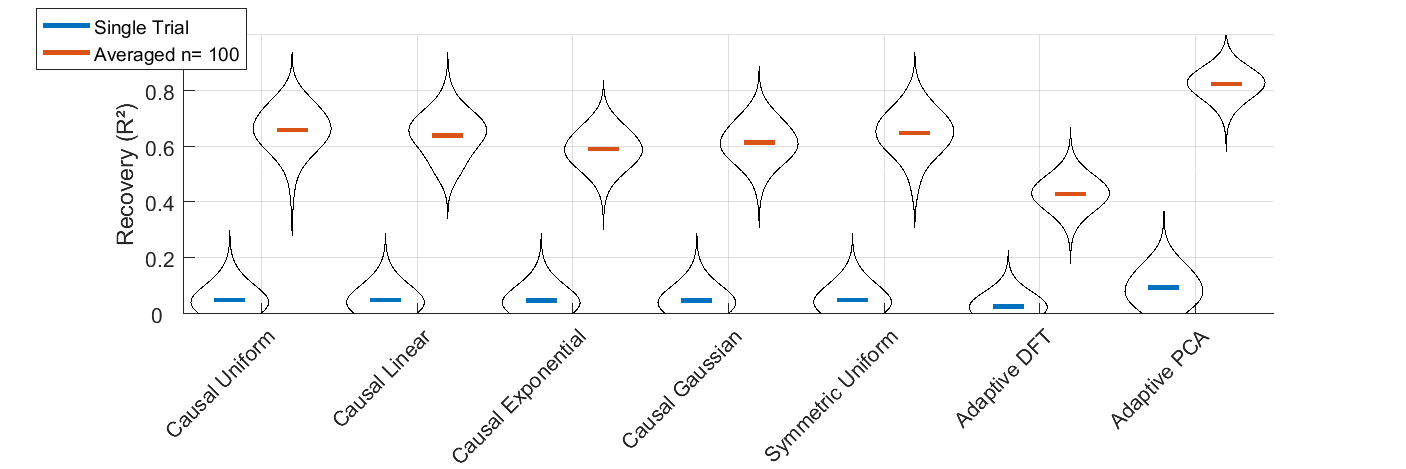
\includegraphics[width=\textwidth]{img/eva/sim_R2.png}
        \caption{Kernel Density Estimation of R² for different filter approaches}\label{fig:simR2}
    \end{subfigure}
    \caption{Overview for Artifact Removal from  Simulated Signal suggests sufficient Performance}
\end{figure}

We simulated 100 trials with a length of 8000 samples. Subsequently, we explored different filters for 10 Hz, all with a period number of 10. The causal DFT filter was applied recursively not only at 10, but also at 20, 30, and 40 Hz to reduce harmonics.

Based on  the correlation of the filtered, artifacted recording with the known shape of the simulated~\gls{erp}, we calculated the R² value. Blue bars indicate the average R² for single-trial reconstructions, and red bars the average R² for boot-strapped grand-average~\gls{erp}s~\figref{fig:simR2}. Visual inspection of the R² estimates shows that all filtering approaches are able to recover at least some information about the~\gls{erp}. Differences between the comb filters is small.

\subsection{Evaluation on real data}\label{sec:EvaluationData}

To evaluate the filters further, we tested them on real physiological signals. Consider that~\gls{tacs} can have physiological effects on cortical~\gls{erp}. To properly evaluate the recovery using the filtering approaches, we needed a physiological signal unlikely to be affected by~\gls{tacs}.

We therefore measured~\gls{ecg} at the flexor digitorum of the left upper limb, while we stimulated distal and proximal with~\gls{tacs} to the recording electrodes~\figref{fig:ecg_setup}. We also recorded~\gls{ecg} at the chest, and detected the R-peak for epoching the data. Please note that no~\gls{tacs}-artifact was visible in the chest~\gls{ecg}.
Physiological signals were acquired using BrainProducts amplifiers at a sampling rate of 1 kHz and low-pass filtered below 35 Hz. Stimulation as delivered using a NeuroConn DC Stimulator Plus with carbon rubber electrodes and Ten20 electrode gel with an intensity of 1 mA at a frequency of 11 Hz.

\begin{figure}[hbtp]
    \begin{subfigure}{.245\textwidth}
        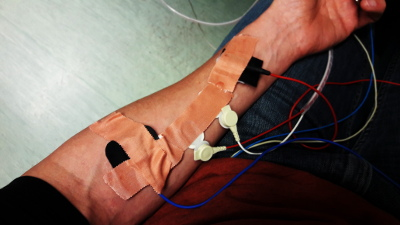
\includegraphics[width=\textwidth]{./img/div/upper_limb_ecg.jpg}
    \caption{Experimental Setup}\label{fig:ecg_setup}
    \end{subfigure}
    \begin{subfigure}{.75\textwidth}
        \begin{subfigure}{.45\textwidth}
            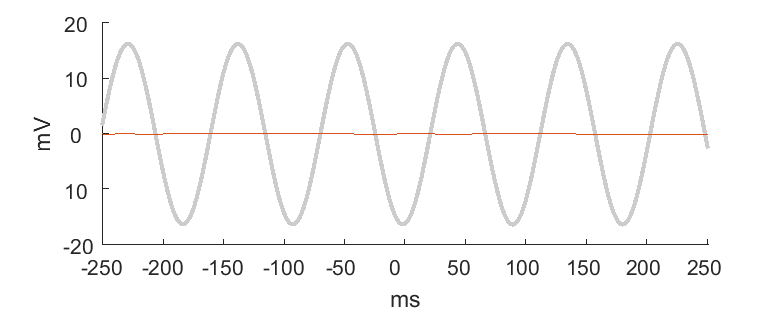
\includegraphics[width=\textwidth]{./img/eva/ecg_raw_1.png}
        \end{subfigure}
        \begin{subfigure}{.45\textwidth}
            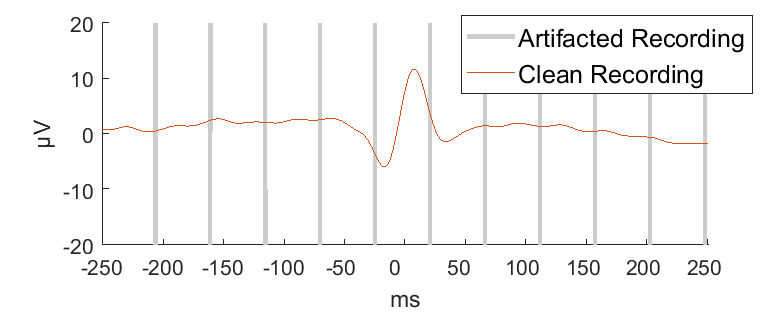
\includegraphics[width=\textwidth]{./img/eva/ecg_raw_2.png}
        \end{subfigure}
    \caption{Signal Comparison}\label{fig:ecgRaw}
    \end{subfigure}
    \begin{subfigure}{1.0\textwidth}
        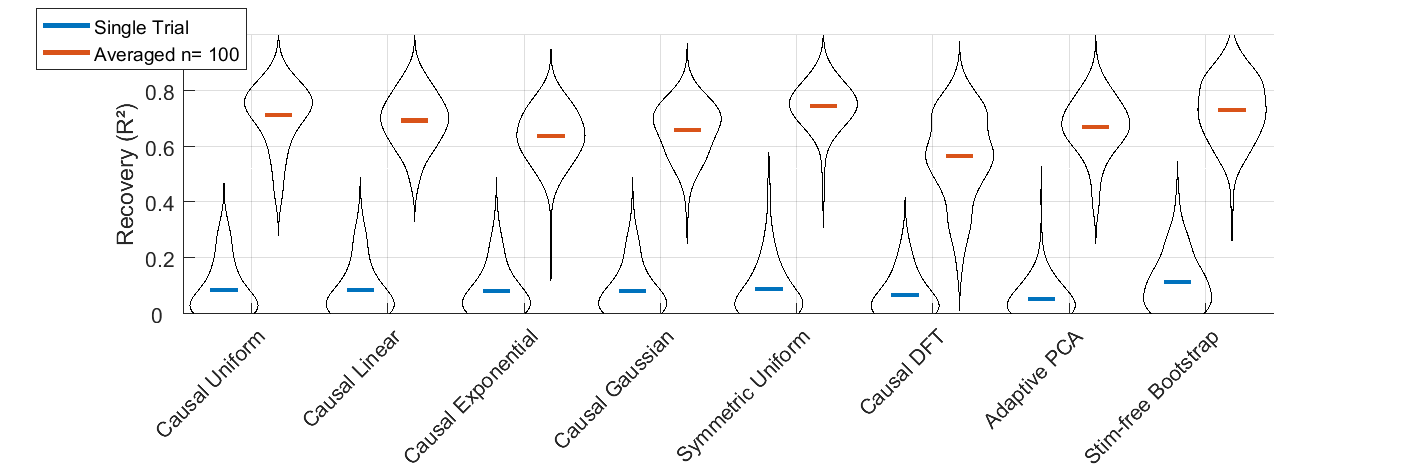
\includegraphics[width=\textwidth]{img/eva/ecg_R2.png}
        \caption{Kernel Density Estimation of R² for different filter approaches}\label{fig:ecgR2}
    \end{subfigure}
    \caption{Overview for Artifact Removal from Upper Limb Electrocardiogram suggests sufficient Performance}
\end{figure}

We detected the R-peak based on the chest-recordings, which allowed us to cut epochs of 8s duration for the recording at the upper limb, for a total of 134 R-peaks without stimulation and 136 with stimulation. We estimated the true shape of the R-peak by taking the average of the stimulation-free signal.
Based on  the correlation of the filtered, artifacted recordings with the averaged stimulation-free recording, we calculated the R² value.
Blue bars indicate the average R² for single-trial reconstructions, and red bars the average R² for boot-strapped grand-average~\gls{erp}s based on 100 epochs~\figref{fig:ecgR2}.
Additionally, note the recovery of the signal in the time-domain~\figref{fig:td_echo}.

\section{Discussion}

We developed a justification for weighted comb filters, and explored their frequency response and their performance on simulated and real data.

\subsection{Performance}\label{sec:discussPerformance}

We found that independent of the weighting function, all comb filters exhibit strong suppression of the DC component, the artifacts frequency and harmonics~\secref{sec:EvaluationSimulated}.
Yet, different weighting functions exhibit different pass-band performance, which is especially evident as ringing~\figref{fig:UniformKernel} or amplification~\figref{fig:ExpTau100}.

For real and simulated datasets, all approaches were able to recover the signal. Contrasting their performance on simulated~\secref{sec:EvaluationSimulated} or real data~\secref{sec:EvaluationData}, we found generally quite similar profiles.

All comb filters performed very similar, but it should be noted that the weighted filters exhibited slightly average lower R² values in both settings and a slightly more skewed distribution for real data~\figref{fig:ecgR2}. This might be linked to distortion by echos~\secref{sec:discussEcho} or insufficient artifact removal in a few trials.
The causal complex filter performed worst, although we filtered not only the main frequency of the artifact, but also the harmonical frequencies. This is most likely caused by the non-sinusoidality of the artifact.

Most interestingly, the causal uniform filter performed on par with the symmetric filters, regardless of whether these were weighted uniform or based on the autocorrelation. This suggests that the causal uniform filter can be highly effective, in spite of its low computational complexity,

The~\gls{ppca} showed superior performance in the simulation, but only average performance in the real dataset. The likely reason is that the linear composition of the simulated recording was a prime candidate for linear separation by~\gls{ppca} and suggests that simulation studies for exploration of filter performance can exaggerate the performance of decomposition approaches.

\subsection{Echos}\label{sec:discussEcho}
A key disadvantage of comb filters is that while they subtract the artifacts, any underlying physiologal signal will cause a periodic echo according to the weights of the kernel.

\begin{figure}[hbtp]
    \begin{subfigure}{0.245\textwidth}
        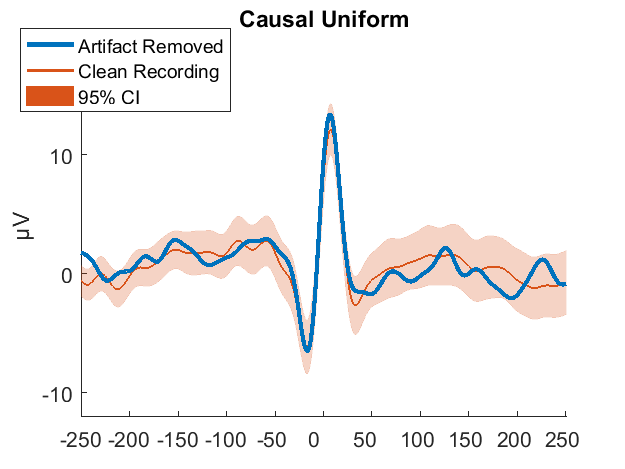
\includegraphics[width=\textwidth]{./img/eva/ecg_td_Causal_Uniform.png}
        \caption{Causal Uniform}\label{fig:td_causaluniform}
    \end{subfigure}
    \begin{subfigure}{0.245\textwidth}
        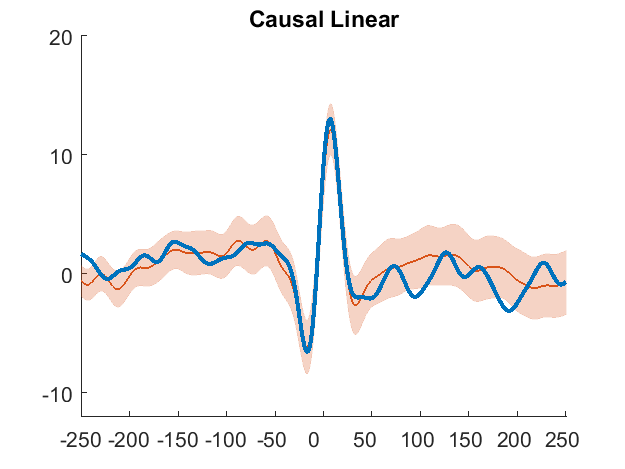
\includegraphics[width=\textwidth]{./img/eva/ecg_td_Causal_Linear.png}
        \caption{Causal Linear}\label{fig:td_causallinear}
    \end{subfigure}
    \begin{subfigure}{0.245\textwidth}
        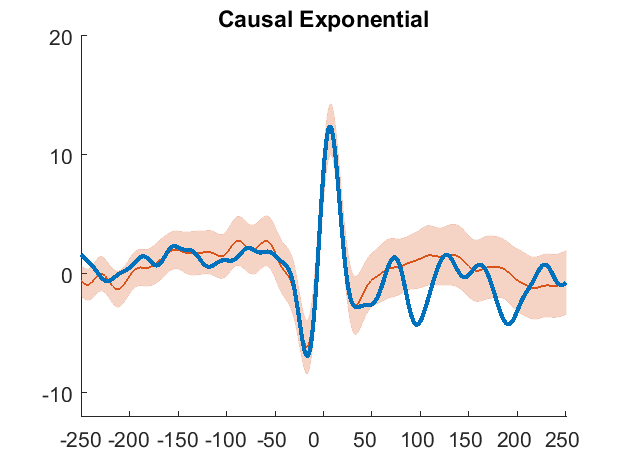
\includegraphics[width=\textwidth]{./img/eva/ecg_td_Causal_Exponential.png}
        \caption{Causal Exponential}\label{fig:td_causalexp}
    \end{subfigure}
    \begin{subfigure}{0.245\textwidth}
        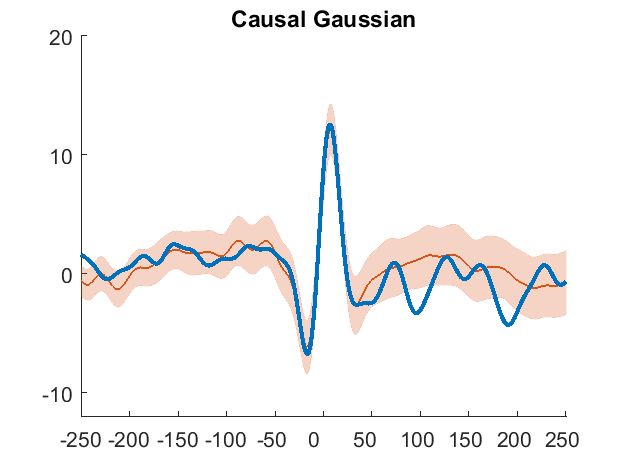
\includegraphics[width=\textwidth]{./img/eva/ecg_td_Causal_Gaussian.png}
        \caption{Causal Gaussian}\label{fig:td_causalgauss}
    \end{subfigure}

    \begin{subfigure}{0.245\textwidth}
        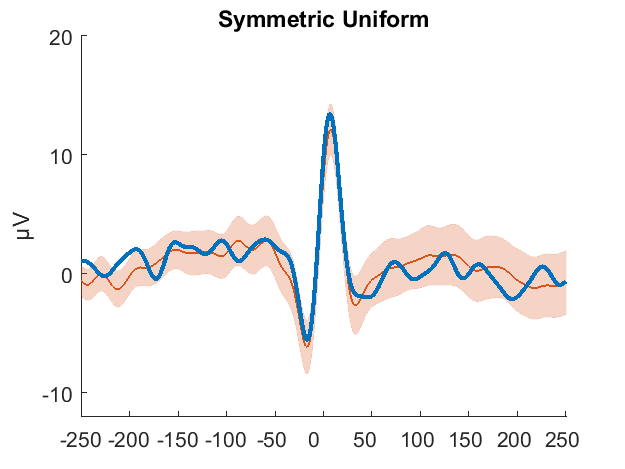
\includegraphics[width=\textwidth]{./img/eva/ecg_td_Symmetric_Uniform.png}
        \caption{Symmetric Uniform}\label{fig:td_symuniform}
    \end{subfigure}
    \begin{subfigure}{0.245\textwidth}
        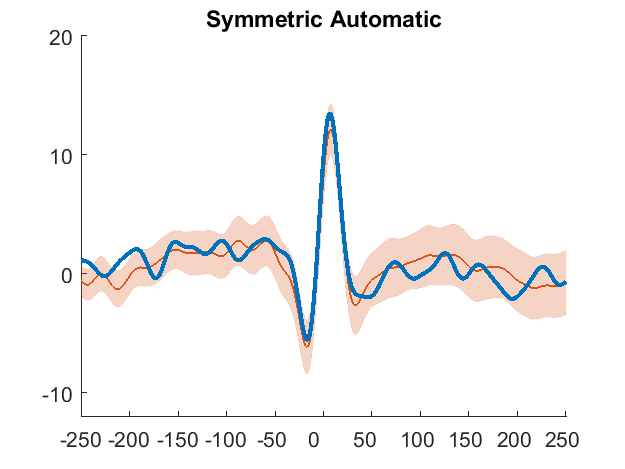
\includegraphics[width=\textwidth]{./img/eva/ecg_td_Symmetric_Automatic.png}
        \caption{Symmetric Automatic}\label{fig:td_symauto}
    \end{subfigure}
    \begin{subfigure}{0.245\textwidth}
        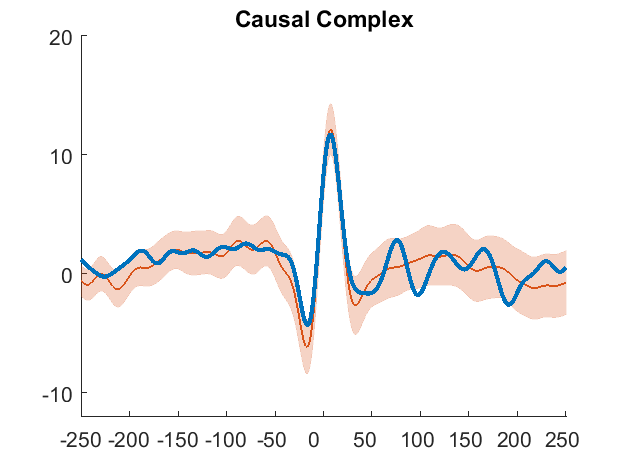
\includegraphics[width=\textwidth]{./img/eva/ecg_td_Causal_Complex.png}
        \caption{Causal Complex}\label{fig:td_causaldft}
    \end{subfigure}
    \begin{subfigure}{0.245\textwidth}
        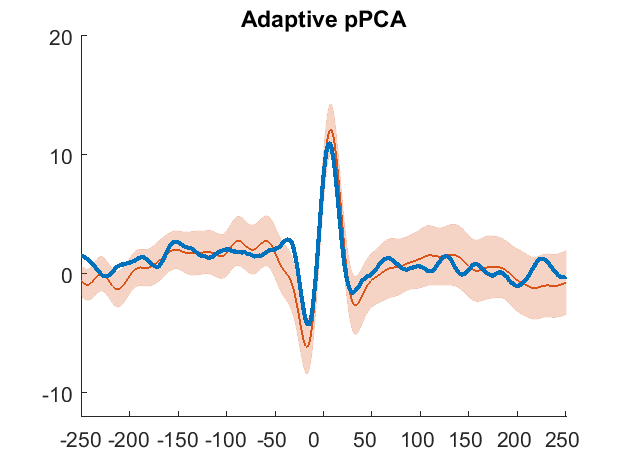
\includegraphics[width=\textwidth]{./img/eva/ecg_td_Adaptive_pPCA.png}
        \caption{Adaptive pPCA}\label{fig:td_pPCA}
    \end{subfigure}
    \caption{Overview of Reconstruction in the time domain highlights possibility of echos}\label{fig:td_echo}
\end{figure}

This means that strong weights close to the kernels center might increase the precision of the artifact amplitude estimate, but can also induce unwanted and strong echos  close to the occurence of a physiologically interesting event~\label{fig:td_echo}.

Additionally, if the duration of the physiological signal is longer than the period of the kernel, the signal will be distorted by the echo.
This could be addressed by~\emph{delaying} the kernel, i.e.\ kernels with zero weights for a number of periods before their estimation weights start, or~\emph{inverting} the kernels, i.e.\ kernels with increasing instead of decreasing weights with increasing delay, or applying causal filters~\emph{piece-wise} left and right of the signal.
~\footnote{If delayed or inverted kernels are used in a symmetric kernel, they appear~\emph{concave}.
While such~\emph{concave, delayed or inverted} kernels might extend the window free of echos around physiological signals, they might not sufficiently account for the non-stationarity of the artifacts amplitude.
The filtered signal might contain a residual artifact.
Whether the trade-off between echo and residual artifact warrants concave kernels depends strongly on the signal under research.
Please note that at least on our datasets and simulations, concave approaches were usually inferior to the regular  causal or symmetric kernels.}

\subsection{Matched Phase and Frequency}

Simulation studies suggested that the power of endogenous oscillations increases if the frequency of~\gls{tacs} matches the targets eigenfrequency~\citep{Kutchko_2013,Zaehle_2010}.
This has been supported by evidence from animal studies~\citep{Schmidt_2014}, and human studies combining \gls{tacs} with \gls{tms} \citep{Guerra_2016}, or contrasting pre and post resting state power analysis \citep{Zaehle_2010}.
It has also been suggested that the phase of neuronal populations would be locked to the phase of the \gls{tacs} signal \citep{Reato_2013}. This has been supported by evidence from studies combining \gls{tacs} with motor output \citep{Brittain_2013}, \gls{tms}~\citep{Raco_2016,Nakazono_2016} or sensory perception~\citep{Gundlach_2016}.
At the same time, event-locked modulation of skin impedance can mimic phase and/or frequency locked modulations. Events might even be endogenous, e.g.\ heart beats~\citep{Noury_2016}.
This suggests that transient and event-locked modulations in frequency and phase matching to the \gls{tacs} can make the  distinction between artifact and neurophysiological effect difficult or impossible.

\subsection{Conclusion}

We note that all filters were able to recover the signal~\figref{fig:ecgR2}, and that the causal uniform filter is comparable to computationally more complex approaches~\secref{sec:discussPerformance}. Pure causal filters with predefined weights can achieve online performance at high speed and with minimal This suggests their utility for environments with limited computational power.

Yet, note that all comb filters exhibit echos, which  can only partially be countered by~\emph{convex} weights. This might limit the applicablity of comb filters to physiological signals with a duration less than one period of the artifact.

Finally, note that comb filters are purely periodic with no assumptions about the shape of the artifact. Comb filters might therefore be useful for filtering of deliberately non-sinusoidal, e.g.\ pulsed~\citep{Jaberzadeh_2015} or misshaped~\citep{Cole_2017} transcranial current stimulation.

\bibliographystyle{apalike-oadoi}
\bibliography{sample}

\end{document}
